\section{Riferimenti teorici}

In questa sezione si forniscono dei riferimenti a basi teoriche necessarie per la comprensione del problema che il progetto punta a risolvere.


\subsection{Rule-Based Systems}

I sistemi di produzione sono un tipo di \emph{Pattern Directed Inference System}. Rappresentano un modello computazionale con regime di controllo guidato da \emph{pattern}. 

Il processo decisionale viene guidato attraverso l'utilizzo di regole: strutture costituite da coppie \emph{antecedente-conseguente}.

La parte \emph{antecedente}, definita anche \emph{LHS} o \emph{condizione}, contiene la rappresentazione di uno schema di caratteristiche che devono corrispondere nella descrizione dello stato corrente del sistema. Nel caso questi schemi (\emph{pattern}) risulteranno verificati, la regola verrà definita \emph{attivabile}. L'attivazione della regola non è immediata, ma gestita in un flusso di controllo ben prestabilito. Con il termine \emph{attivazione} verrà definita la coppia formata da una \emph{regola attivabile} e l'insieme di caratteristiche presenti nella descrizione dello stato che hanno reso la regola \emph{attivabile}.

La parte \emph{conseguente}, definita anche \emph{RHS} o \emph{azione}, rappresenta l'azione (o l'insieme di azioni) che dovranno essere eseguite nel momento in cui una regola \emph{attivabile} verrà effettivamente attivata. Solitamente il gruppo conseguente consiste in una serie di modifiche da apportare alla descrizione dello stato del sistema, ma questa generalizzazione non rappresenta una restrizione.

Il funzionamento di questa classe di sistemi può essere espresso come una sequenza di cicli \emph{recognize-act}:
\begin{description}
	\item[recognize:] viene valutata l'applicabilità di ogni regola in relazione allo stato corrente del sistema. La valutazione viene effettuata confrontando lo stato del sistema con la porzione \emph{LHS} di ogni regola.
	\item[selezione:] vengono applicati dei principi di selezione per individuare una o più regole fra quelle attivabili. L'insieme di principi utilizzati viene definito con il nome di \emph{strategia di risoluzione di conflitti}.
	\item[act:] la regola selezionata viene attivata: l'elenco di azioni presenti nella porzione \emph{RHS} vengono eseguite.
\end{description}

\'E evidente come il ciclo sia strutturato in modo che il momento di esame dei dati sia nettamente separato dal momento di elaborazione o modifica degli stessi. Inoltre l'unica modalità per lo scambio di informazioni fra le regole prevista, avviene attraverso la modifica stessa dello stato del sistema presente nella \emph{working memory}. Questa caratteristica differenzia ulteriormente questa classe di sistemi da quelli con approccio procedurale: se l'approccio basato su regole di produzione prevede che la stessa descrizione dello stato sia condivisa fra tutte le regole e che l'accesso allo stesso sia garantito in egual misura, il modello procedurale prevede che le singole procedure accedano ad un ristretto (e focalizzato) sottoinsieme dei dati presenti nello stato globale.

\subsubsection{Componenti di un RBS}


La struttura classica di un sistema basato su regole può essere schematizzata (\figurename~\ref{fig:architettura-rbs}) attraverso la specifica dei quattro componenti principali da cui è composto.

\begin{figure}[h]
\centering
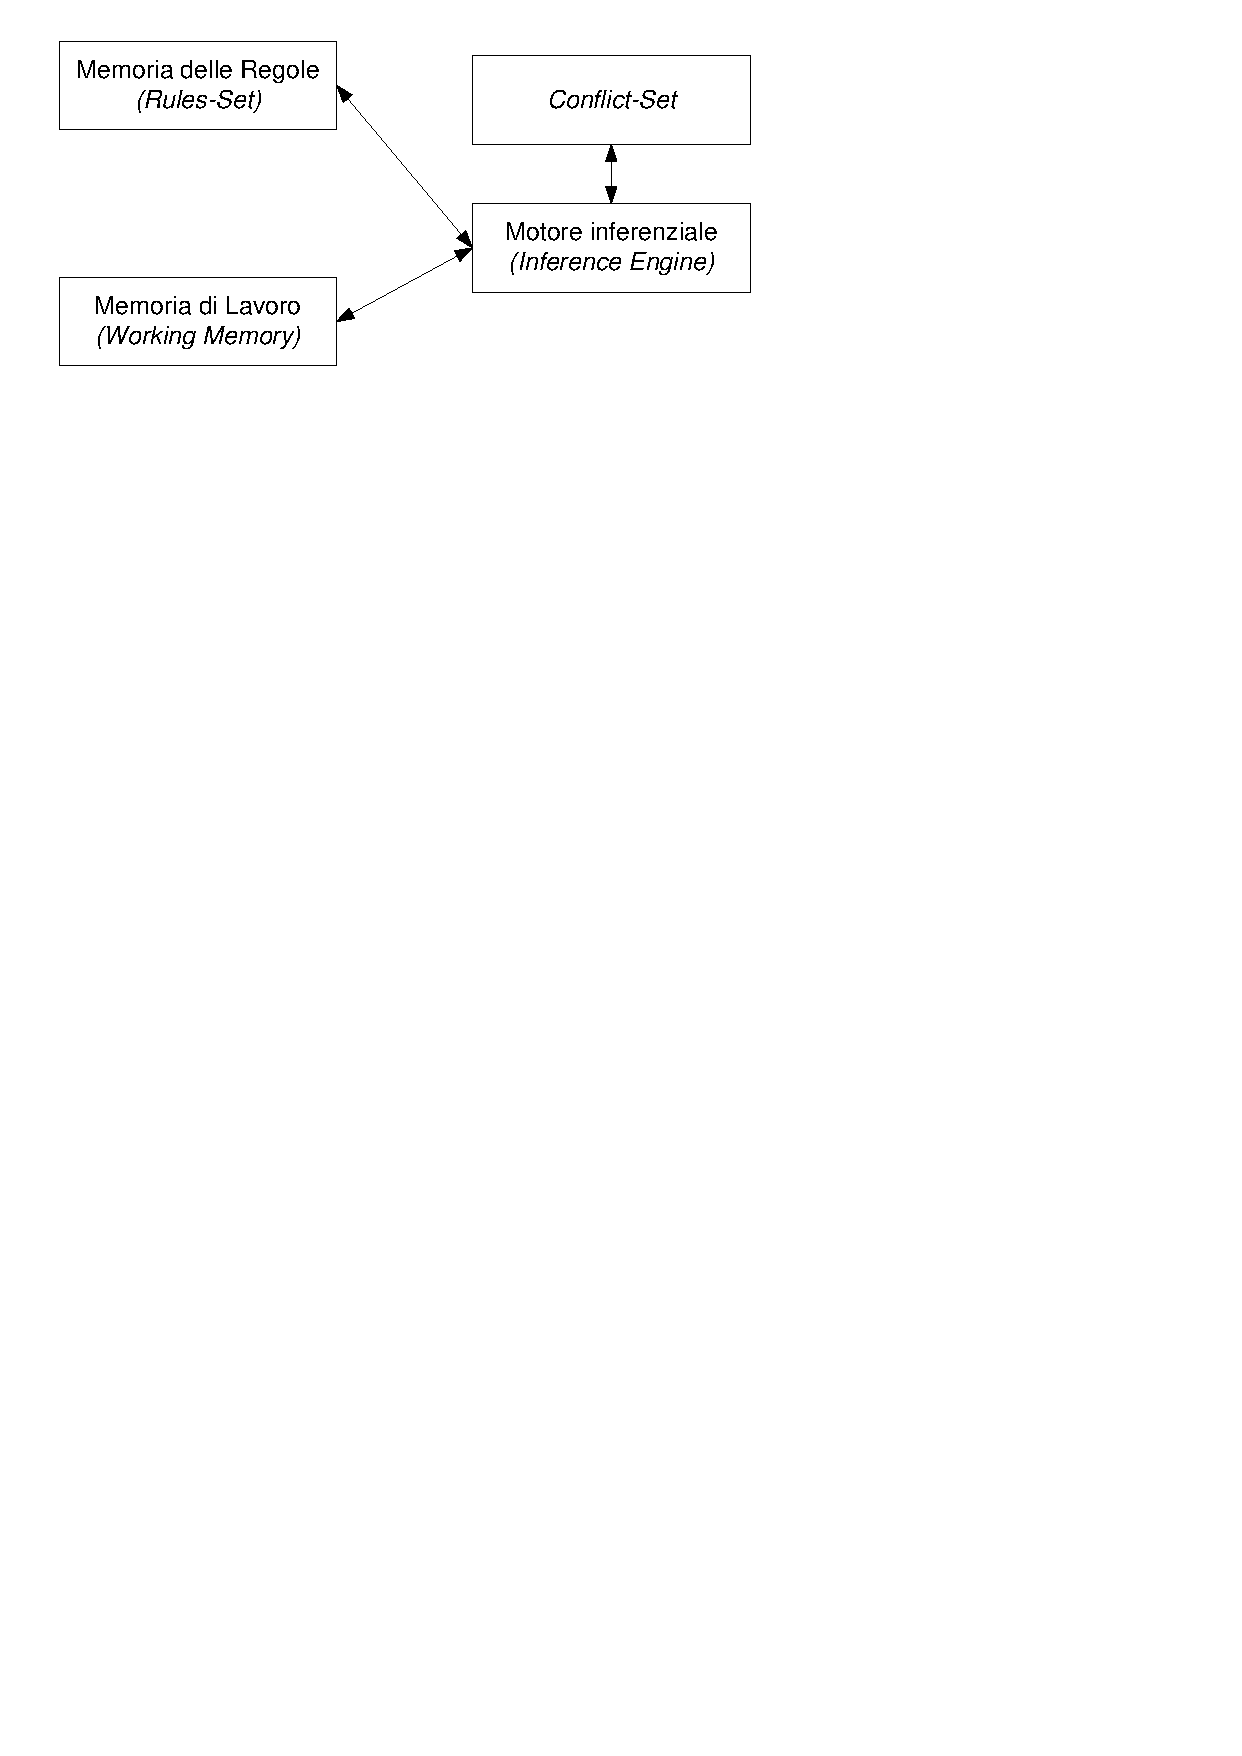
\includegraphics[viewport=28 667 361 824]{Immagini/Capitolo2/Architettura-RBS.pdf}
\caption{Architettura generalizzata di un Rule-Based System}\label{fig:architettura-rbs}
\end{figure}

\subparagraph{Memoria di lavoro}
La memoria di lavoro, anche chiamata \emph{working memory}, è il componente destinato ad accogliere la descrizione simbolica dello stato del sistema. La descrizione è composta da strutture simboliche note con il nome di \emph{fatti}. La forma con la quale i fatti vengono rappresentati dipende dal sistema spesso, ma formalismi comunemente utilizzati prevedono una rappresentazione tramite \emph{vettori di caratteristiche} o \emph{triple (oggetto, proprietà, valore)}.

La \emph{working memory} viene utilizzata dal motore inferenziale per il processo di verifica della possibilità di attivazione delle regole.

\subparagraph{Motore inferenziale}

Il \emph{motore inferenziale}, o \emph{inference engine}, rappresenta il nucleo centrale di ogni sistema a regole: è il componente con il compito di valutare la parte \emph{LHS} delle regole, identificare quelle attivabili compilando il \emph{conflict-set} e infine, in seguito ad un processo di selezione guidato dalla \emph{strategia di risoluzione dei conflitti}, eseguirne una.

Il processo alla base della valutazione delle regole applicabili prende il nome di \emph{pattern-matching}.

\subparagraph{Memoria delle regole}
La memoria delle regole, o \emph{rules-set}, è una struttura che conserva l'insieme di regole definite nel sistema. Viene consultata dal motore inferenziale per individuare le regole attivabili per uno stato del sistema.

\subparagraph{Conflict-Set}
Il \emph{conflict-set}, anche noto in determinati sistemi con il nome di \emph{agenda} o \emph{agenda delle attivazioni}, è un componente che conserva l'insieme di \emph{attivazioni} disponibili per lo stato corrente della \emph{working-memory}. L'insieme viene compilato dal \emph{motore inferenziale} al termine del passo \emph{recognize} che caratterizza questa classe di sistemi.

Il \emph{conflict-set} viene consultato per effettuare una selezione nell'insieme di attivazioni disponibili, utilizzando una \emph{strategia di risoluzione dei conflitti}, e individuare l'attivazione da eseguire nel passo \emph{act}.

\subsection{Unificazione e Pattern Matching}\label{par:pattern-matching}

Il problema del \emph{confronto di descrizioni simboliche} è uno dei problemi alla base dei sistemi basati su conoscenza. Una forma di questo genere di problemi è quello dell'\emph{unificazione} o \emph{matching}.

L'\emph{unificazione} rappresenta un procedimento con il quale vengono confrontate fra loro un insieme di due o più strutture simboliche per identificarne differenze o somiglianze.~\cite{ferilli200}

Dati due termini $s$ e $t$, il problema dell'unificazione consiste nel capire se esistono dei termini in grado di essere sostituiti alle variabili che compaiono in $s$ e $t$ affinché i termini ottenuti risultino identici.~\cite{ferilli200}

Per molte applicazioni pratiche, l'unificazione risulta un concetto troppo generale. Si fa quindi riferimento al \emph{Pattern Marching}, una variante dell'unificazione nella quale è possibile effettuare sostituzioni solo in una delle due strutture simboliche.~\cite{ferilli200}


\begin{defn}[Termini confrontabili]
Dati due termini, $s$ e $t$, si dice che \emph{esiste un matching} tra essi se esiste una sostituzione $\mu$ tale che:
\begin{equation}
\mu(s)=t \text{ oppure } \mu(t)=s
\end{equation}
In tal caso $\mu$ è definito \emph{matcher} di $s$ e $t$, mentre $\mu(s)$ (risp. $\mu(t)$) è definito \emph{matching} di $s$ e $t$.
\end{defn}

\subsection{Strategie di risoluzione dei conflitti}\label{par:strategies}

Come visto in precedenza, la fase \emph{recognize} ha lo scopo di valutare eventuali cambiamenti apportati allo stato del sistema identificando l'insieme di \emph{attivazioni} disponibili. L'elenco di \emph{attivazioni} verrà memorizzato nel \emph{conflict-set}. 

In una fase successiva, l'utilizzo di determinate euristiche provvederà a definire dei criteri con i quali discriminare l'insieme di attivazioni per identificarne un sotto-insieme\footnote{Solitamente composto di un solo elemento.}.

L'insieme di criteri con i quali discriminare l'insieme prende il nome di \emph{strategia di risoluzione dei conflitti}.

\subsection{CLIPS}\label{par:clips}

CLIPS (C Language Integrated Production System) è uno dei più conosciuti \emph{Expert System Environment}. Implementato in linguaggio C presso i laboratori NASA del Johnson Space Center, è attualmente uno dei sistemi più utilizzati in ambito accademico grazie alla sua reperibilità e gratuità.

CLIPS è un ambiente multi-paradigmatico che integra all'interno di un'architettura di base di tipo \emph{RBS}, elementi per la programmazione procedurale e orientata ad oggetti.

L'interazione con il sistema può avvenire attraverso l'utilizzo di una \emph{Shell}, che consente l'immissione di costrutti, l'esecuzione di query e chiamate a funzioni, oppure attraverso l'integrazione del sistema in applicazioni classiche, che ne sfruttino i servizi tramite apposite API.

Il sistema prevede dei meccanismi di estensione tramite la compilazione congiunta di funzioni in linguaggio C, le quali verranno rese disponibili nel sistema in maniera analoga a quelle integrate in origine.

\subsubsection{Presentazione dei formalismi di specifica}\label{par:clips-formalism}

Il linguaggio di specifica utilizzato da CLIPS, prevede una sintassi simile a quella utilizzata da LISP. La definizione dei costrutti (\emph{regole}, \emph{template}, \emph{funzioni}, \emph{fatti}, $\dots$) avviene utilizzando un linguaggio chiamato CLIPS, analogamente al sistema. Un'estensione del linguaggio fornito originariamente, che prende il come di \emph{COOL}, è stata aggiunta nelle versioni successive per integrare il supporto il paradigma \emph{object-oriented}.

\paragraph{Moduli}
Per consentire il riuso e agevolare lo sviluppo incrementale dei sistemi esperti, oltre che per agevolare la specifica di meccaniche di tipo \emph{goal-directed}, CLIPS prevede la definizioni di moduli e un protocollo per la condivisione delle definizioni dei costrutti fra più moduli.

\begin{program}
\begin{verbatimtab}

(defmodule A
	(export ?ALL))

(defmodule B
	(import A ?ALL))
\end{verbatimtab}
\caption{Esempio d'uso di \emph{defmodule} per la specifica di moduli}
\end{program}

La definizione dei moduli avviene utilizzando il costrutto \emph{defmodule}. La sintassi prevede la possibilità di specificare un elenco di costrutti da rendere disponibili ad altri moduli (tramite l'attributo \emph{export}), oppure un elenco di definizioni da importare da un modulo precedentemente creato (tramite l'attributo \emph{import}).

Il meccanismo di \emph{import/export} è una delle caratteristiche principali del sistema di moduli fornito da CLIPS. Consente in questo modo di introdurre un meccanismo di \emph{information hiding} e rendere più facile in riuso di moduli indipendenti.

\paragraph{Funzioni utente}
L'utente, in maniera alternativa all'integrazione di funzioni native scritte in linguaggio C, può aggiungere funzioni personalizzate all'interno del sistema utilizzando il costrutto \emph{deffunction}.

\begin{program}
\begin{verbatimtab}

(deffunction Funzione_Di_Prova (?arg1)
	(printout t ?arg1 crlf)
)
\end{verbatimtab}
\caption{Esempio d'uso di \emph{deffunction} per la specifica di funzioni}
\end{program}


Le funzioni cosi integrate potranno essere utilizzate nelle stesse modalità previste dalle altre funzioni di sistema, con l'eccezione relativa ai vincoli di visibilità fra moduli.

\begin{program}
\begin{verbatimtab}

(defmodule A
	(export deffunction Funzione_Di_Prova))
	
(deffunction A::Funzione_Di_Prova () )

(defmodule B
	(import A deffunction Funzione_Di_Prova))
\end{verbatimtab}
\caption{Esempio di esportazione della definizione di una funzione}
\end{program}

Le definizioni di funzioni devono essere esportate dal modulo in cui sono definite e successivamente importate da quello che, invece, intende utilizzarle.

\paragraph{Regole}
Componente chiave di ogni \emph{RBS}, la specifica delle regole può essere effettuata utilizzando il costrutto \emph{defrule}.

\begin{program}
\begin{verbatimtab}

(defrule Make_Bird_Fly
	(bird (type ?X))
	=>
	(assert (bird (type ?X)	(fly yes)))
)
\end{verbatimtab}
\caption{Esempio d'uso di \emph{defrule} per la specifica di una regola}\label{code:defrule}
\end{program}

L'attivabilità della regola è soggetta, oltre che a vincoli relativi dal normale processo di \emph{pattern-matching}, anche a vincoli derivanti dal modulo in cui il processo è focalizzato.

Come mostrato in Codice~\ref{code:defrule}, la porzione \emph{LHS} e \emph{RHS} della regola sono separati dal simbolo $=>$. La regola definizione i \emph{pattern} della \emph{LHS} usando i formalismi \emph{Ordered-Fact} e \emph{Template-Fact}. I \emph{pattern} possono essere accorpati e specificati in aggiunta a modificatori come \emph{exists}, \emph{not}, \emph{or}, $\dots$.

La porzione \emph{RHS} contiene chiamate a procedure di sistema o definite dall'utente tramite il costrutto \emph{deffunction}.

\paragraph{Fatti}

I \emph{fatti}, insieme alle \emph{instanze}, costituiscono il contenuto della \emph{working memory}. L'asserzione o ritrattazione dei fatti avviene attraverso l'utilizzo della funzioni di sistema \emph{assert} e \emph{retract}. Altre funzioni che interagiscono con la \emph{memoria di lavoro} con modalità simili, ma effetti leggermente differenti, sono \emph{modify} e \emph{duplicate}.

L'utilizzo di queste funzioni avviene congiuntamente all'utilizzo di una delle due possibili notazioni per la specifica dei fatti.

\begin{program}
\begin{verbatimtab}

(deffacts Fatti_Iniziali
	(A B C)
	(bird (type penguin))
	(bird (type eagle))
	(combattente
		(mano-sx pugnale)
		(mano-dx tomahawk)
		(cintura scalpo scalpo scalpo))
)
\end{verbatimtab}
\caption{Definizione di un gruppo di fatti tramite \emph{deffacts}}\label{code:deffacts}
\end{program}


Una possibilità alternativa di specifica dei fatti iniziali è quella prevista tramite l'utilizzo del costrutto \emph{deffacts}. Il costrutto consente di inserire un elenco di definizioni che verranno automaticamente asserite durante la fase di inizializzazione del sistema esperto.

\begin{program}
\begin{verbatimtab}

(A B C)
\end{verbatimtab}
\caption{Fatto definito utilizzando la notazione \emph{Ordered-Fact}}\label{code:ordered-fact}
\end{program}

La prima, chiamata \emph{Ordered-Fact}, prevede la definizione di fatti come vettori di elementi simbolici o numerici di lunghezza definita. Il formato del primo elemento è richiesto che sia di tipo \emph{SYMBOL}\footnote{SYMBOL rappresenta un tipo elementare presente in CLIPS. Appartengono a questo tipo tutte le sequenze alfanumeriche non delimitate da apici e che abbiano come primo elemento un carattere alfabetico}, il formato dei successivi elementi è arbitrario.

\begin{program}
\begin{verbatimtab}

(combattente
	(mano-sx scudo)
	(mano-dx spada)
	(cintura carne-secca borraccia monete))
\end{verbatimtab}
\caption[Fatto definito utilizzando la notazione \emph{Template-Fact}]{Fatto definito utilizzando la notazione \emph{Template-Fact}. Il nome del template a cui il fatto fa riferimento è \emph{combattente}. La specifica del \emph{template} prevede l'esistenza degli slot ''mano-sx'', ''mano-dx'' e ''cintura''}\label{code:template-fact}
\end{program}

La seconda modalità di specifica, denominata \emph{Template-Fact}, prevede la definizione dei fatti tramite l'utilizzo di un \emph{template} e una sequenza di \emph{slot}. Gli slot rappresentano delle caratteristiche definite nella specifica di \emph{template}.
La definizione del fatto può prevedere la specifica di tutti o solo una porzione degli \emph{slot} previsti dal \emph{template}. CLIPS prevede la possibilià di definire dei valori di \emph{default} da applicare in caso di mancato avvaloramento di uno slot.
I valori inseribili negli \emph{slot} possono essere singoli elementi o multipli. Nel secondo caso si farà riferimento allo \emph{slot} con il nome di \emph{multi-slot} (un esempio è quello fornito dal \emph{multi-slot} ''cintura'' dell'esempio in Codice~\ref{code:template-fact}).

\paragraph{Template}
La specifica dei fatti in formato \emph{Template-Fact} prevede la definizione preventiva di un \emph{template} che definisca una ''tipologia'' di fatti, indicandoli con un nome univoco, e una sequenza di caratteristiche, esplicitando utilizzando \emph{slot} e \emph{multi-slot}.

\begin{program}
\begin{verbatimtab}

(deftemplate combattente "rappresenta un combattente"
	(slot mano-sx 
		(type SYMBOL))
	(slot mano-dx
		(default spada)
		(type SYMBOL))
	(multislot cintura))
\end{verbatimtab}
\caption{Specifica di \emph{Template} tramite \emph{deftemplate}}\label{code:deftemplate}
\end{program}

L'esempio fornito in Codice~\ref{code:deftemplate} rappresenta una possibile definizione di \emph{template} valida per il fatto in Codice~\ref{code:template-fact}.

La specifica prevede la definizione di valori di \emph{default} (come ad esempio per lo \emph{slot} ''mano-dx''), da attribuire nei casi in cui non venga fornito un valore durante l'asserzione, oppure di restrizioni sul tipo di valore memorizzabile nello \emph{slot}.

\subsection{Architetture per sistemi distribuiti}

Un sistema distribuito consiste di una collezione di componenti, distribuiti su diversi terminali (anche chiamati \emph{host}) connessi fra loro attraverso una rete. Questi componenti interagiscono fra loro al fine di scambiare dati od accedere reciprocamente a servizi disponibili.~\cite{Mascolo:2002:MCM:770420.770423}

Ad alto livello, la realizzazione di un sistema distribuita è soggetta alla predisposizione di un sistema di comunicazione in grado di mettere in comunicazione i processi distribuiti fra i vari \emph{host}.

Sono disponibili diverse architetture per strutturare un sistema distribuito. Le più note prendono i nomi di \emph{Client-Server}, \emph{3-tier Architecture}, \emph{n-tier Architecture}, \emph{Peer-to-Peer}, solo per citarne alcune.

\subsubsection{Modello Client-Server}
Il modello di architettura \emph{Client-Server} si basa sul partizionamento delle attività, risorse e responsabilità del sistema in due classi di componenti: \emph{Server} e \emph{Client}.

I componenti possono essere distribuiti su diversi \emph{host}, così come possono essere collocati in processi separati residenti sulla stessa macchina in modo che non condividano direttamente risorse (\figurename~\ref{fig:client-server}). Lo scambio di informazioni avviene attraverso un protocollo stabilito e noto ad entrami i sistemi.

\begin{figure}[h]
\centering
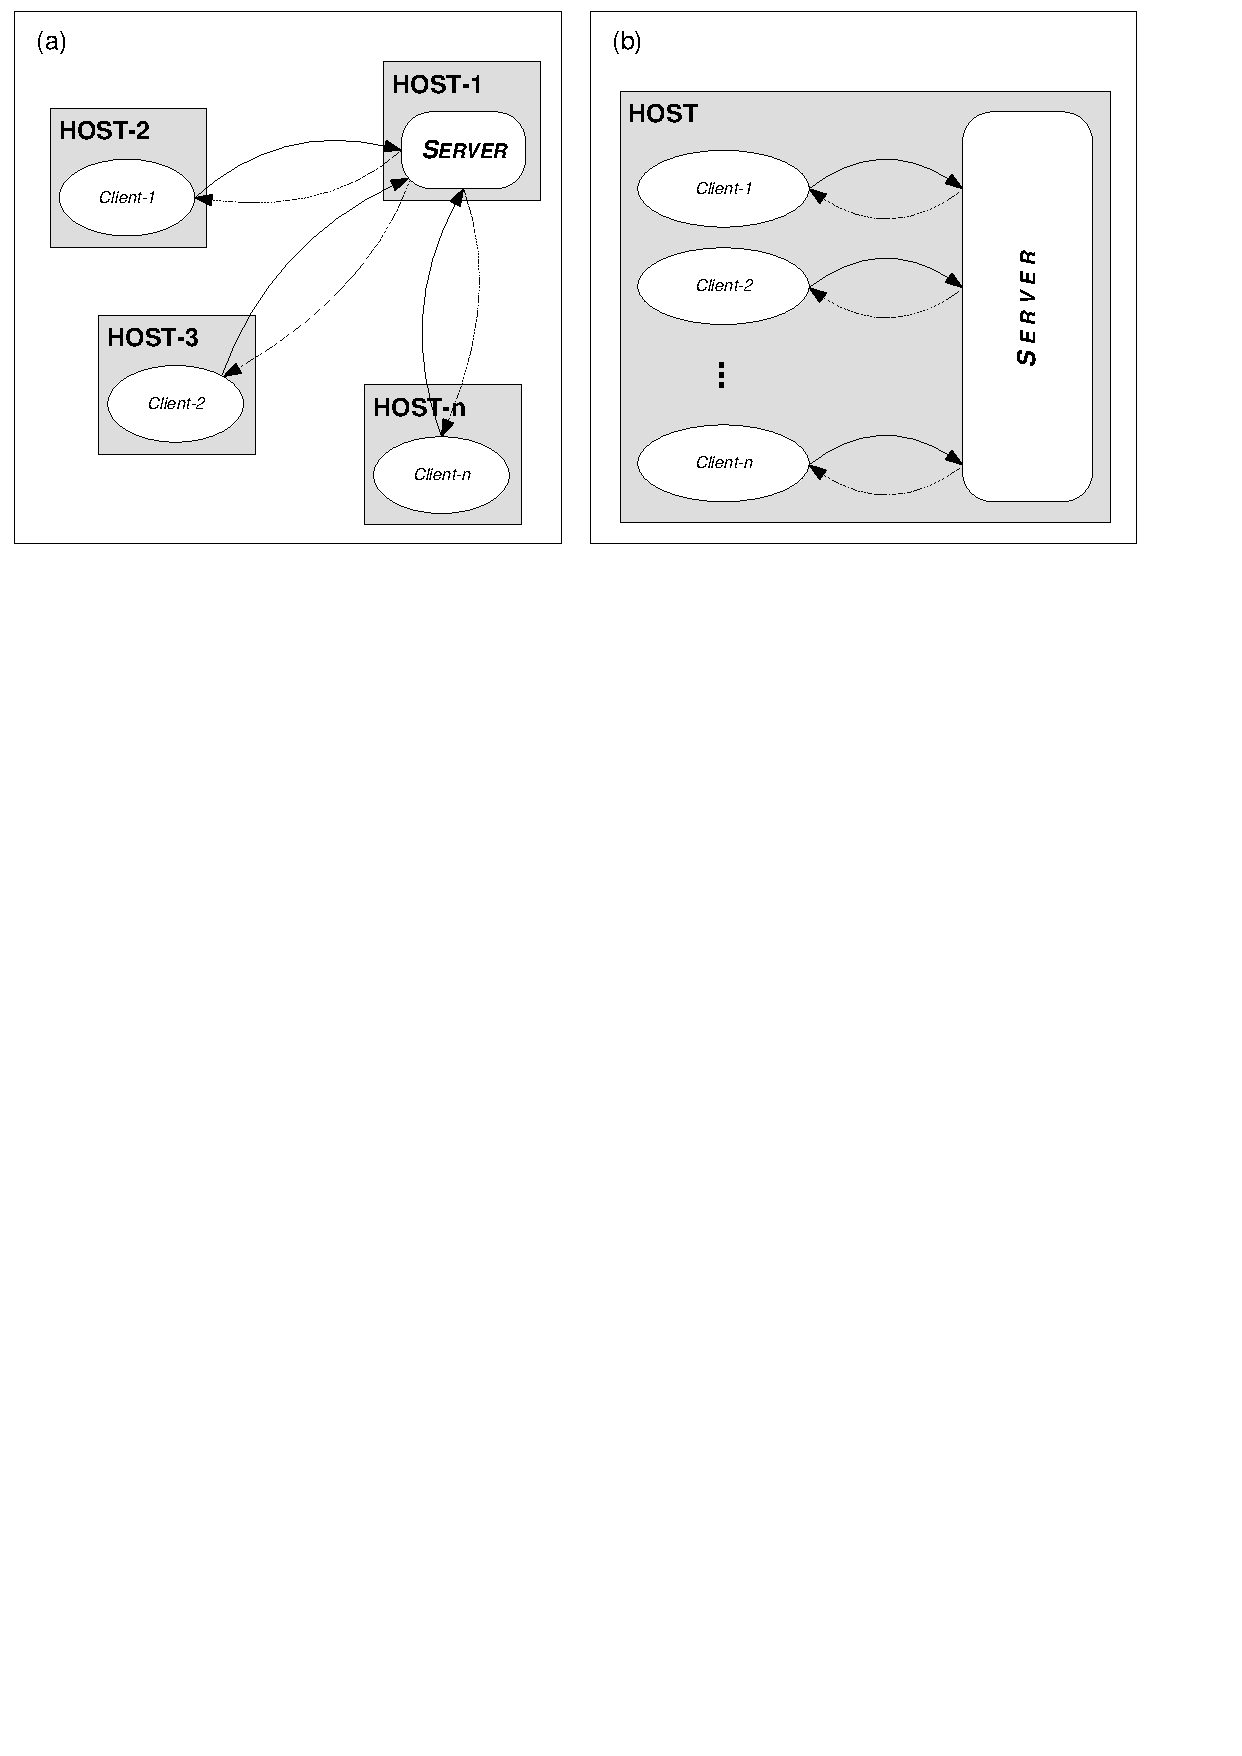
\includegraphics[scale=0.7, viewport=6 582 546 838]{Immagini/Capitolo2/Client-Server.pdf}
\caption[Architettura \emph{Client-Server}]{Architettura \emph{Client-Server}: in \emph{(a)} è mostrata una distribuzione su \emph{host} multipli, in \emph{(b)} una distribuzione in processi multipli}\label{fig:client-server}
\end{figure}

L'architettura \emph{Client-Server} descrive un modello di collaborazione fra sistemi. Il \emph{server} offre servizi o funzionalità a uno o più \emph{client}, mentre il \emph{client} effettua una richiesta e, solitamente, provvede ad elaborare i dati ottenuti come risposta dal \emph{server} per presentarli all'utente o proseguire con ulteriori elaborazioni.

\subsubsection{Protocollo XML-RPC}\label{par:xmlrpc}

\emph{Remote Procedure Call}, o \emph{RPC}, è un meccanismo tramite il quale un'applicazione posizionata su una \emph{macchina} richiede l'utilizzo di servizi forniti da un'altra applicazione residente su una \emph{macchina} differente. Con il termine \emph{macchina} non viene unicamente inteso un \emph{host}, un'installazione fisicamente indipendente, ma anche un processo residente in una porzione di memoria indipendente e che rende l'accesso alle risorse del servizio impossibile se non tramite il meccanismo \emph{RPC}. 

Il meccanismo \emph{RPC} prevede che una prima applicazione possa inviare uno o più messaggi ad una applicazione differente per invocare delle procedure. L'applicazione ricevente ha la possibilità,  a sua volta, di inviare i risultati dell'elaborazione tramite un ulteriore messaggio verso applicazione richiedente.~\cite{MERRICK:2006:misc}

\emph{RPC} descrive un meccanismo generalizzato per l'invocazione di procedure remote, non una concreta implementazione di un protocollo o di tecnologie per lo scambio dei messaggi fra gli \emph{host}. Partendo dal concetto generale di \emph{RPC}, nel tempo sono state proposte differenti implementazioni basate su protocolli proprietari o codifiche dei messaggi differenti.~\cite{JAIRATH:2004:misc}~\cite{dcerpc}

\emph{XML-RPC} è una fra le implementazioni proposte per \emph{RPC}: si propone come un meccanismo di chiamata a procedura remote semplice e versatile. Il brevetto originale con il quale è stato proposto descrive sia il meccanismo di chiamata, che un sistema per l'implementazione del metodo.~\cite{MERRICK:2006:misc}

\begin{figure}[h]
\centering
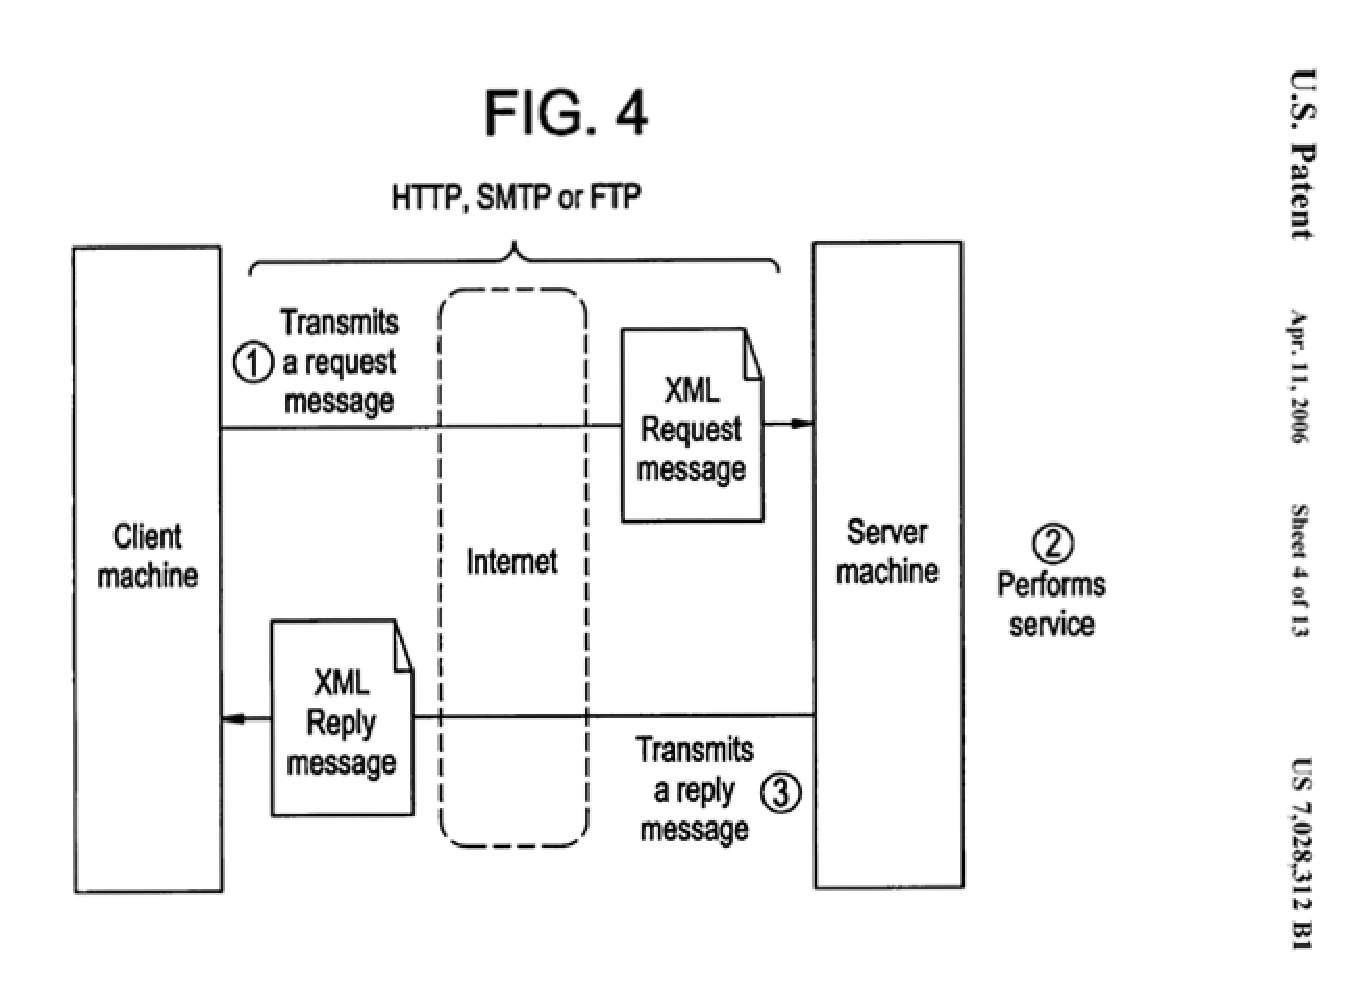
\includegraphics[scale=0.5, viewport=0 0 646 440]{Immagini/Capitolo2/XMLRPC-patent.pdf}
\caption[Comunicazione tramite \emph{XML-RPC}]{Comunicazione tramite \emph{XML-RPC}: immagine presente nella richiesta originale di brevetto~\cite{MERRICK:2006:misc}.}\label{fig:xmlrpc-patent}
\end{figure}

\emph{XML-RPC} prevede lo scambio di richieste e risposte usando il formato \emph{XML}, attraverso meccanismi di trasporto multipli. Solitamente, con l'uso del termine \emph{XML-RPC} si è soliti però indicare il protocollo di scambio messaggi in \emph{XML} attraverso un meccanismo di trasporto basato sul protocollo \emph{HTTP}.

\begin{program}
\begin{verbatimtab}

POST /RPC2 HTTP/1.0
User-Agent: Frontier/5.1.2 (WinNT)
Host: betty.userland.com
Content-Type: text/xml
Content-length: 181


<?xml version="1.0"?>
<methodCall>
   <methodName>examples.getStateName</methodName>
   <params>
      <param>
         <value><i4>41</i4></value>
         </param>
      </params>
   </methodCall>
\end{verbatimtab}
\caption{Esempio di chiamata ad una procedura remota usando \emph{XML-RPC over HTTP}}\label{code:xmlrpc-request}
\end{program}

La codifica dei messaggi viene effettuata incapsulando i parametri di chiamata ed i valori di ritorno all'interno di appositi frammenti del documento \emph{XML}, i quali hanno il compito di attribuire una semantica alla stringa rappresentante il valore.

\begin{program}
\begin{verbatimtab}
HTTP/1.1 200 OK
Connection: close
Content-Length: 158
Content-Type: text/xml
Date: Fri, 17 Jul 1998 19:55:08 GMT
Server: UserLand Frontier/5.1.2-WinNT


<?xml version="1.0"?>
<methodResponse>
   <params>
      <param>
         <value><string>South Dakota</string></value>
         </param>
      </params>
   </methodResponse>
\end{verbatimtab}
\caption{Esempio di messaggi inviato a risposta di una chiamata a procedura remota usando \emph{XML-RPC over HTTP}}\label{code:xmlrpc-response}
\end{program}

I \emph{tag} che contengono il valore ne determinano il tipo. Nell'esempio fornito in Codice~\ref{code:xmlrpc-request}, il valore ''41'' (tipo \emph{integer}) viene incapsulato nel \emph{tag i4}. Il tag indica appunto che il tipo del valore, come da specifica, è un \emph{4 bytes signed integer}.

La specifica prevede la possibilità di utilizzare un set di tipi atomici con i quali rappresentare tutti i parametri di chiamata a procedura o i valori di ritorno (''integer'', ''string'', ''boolean'', ''double'', ''dateTime.iso8601'', ''base64'') e un gruppo di strutture composte (''struct'' per strutture analoghe a dizionari, ''array'' per vettori).~\cite{xmlrpcspec}
